\newpage
\appendix

\section{Latency Model for LLM Inference}
\label{appendix:latency_model}

To accurately simulate the goodput of different placement strategies, we use an analytical model to predict the execution time of the prefill and decoding phases in LLM inference. 

In modern LLM serving systems~\cite{fastertransformer, vllm, wu2023fast}, memory-bound operations like Softmax and LayerNorm are usually fused with matrix multiplication kernels for efficiency. Thus the GEMMs dominate the overall latency and our analysis primarily focuses on them. 

\subsection{Symbol Definition}

Here are symbols related to the architecture of the model:

\begin{itemize}
    \item $h$: hidden size
    \item $n$: number of heads
    \item $s$: head size ($h = n \cdot s$)
    \item $m$: FFN intermediate size
\end{itemize}

Note: If tensor parallelism is used, $h$, $n$, and $m$ should be divided by the tensor parallelism size.

Below are symbols that characterize the batch to be executed:

\begin{itemize}
    \item $B$: batch size
    \item $l_0, l_1, \dots, l_{B-1}$: input length of each request within the batch
    \item $t$: number of tokens in the batch, ($t = \sum_{i=0}^{B-1} l_i$)
    \item $t_2$: squared sum of the input lengths ($t_2 = \sum_{i=0}^{B-1} l_i^2$)
    \item $b$: block size in the attention kernel. This parameter is used in FlashAttention~\cite{dao2022flashattention}, a common kernel optimization technique adopted by current LLM serving systems.
\end{itemize}


\subsection{Prefill Phase Latency Modeling}

Since the attention operation uses specially optimized kernels, we first discuss the other four matrix multiplications in the prefill phase:

\begin{table}[h]
\centering
\begin{tabular}{|c|c|c|}
    \hline
    GEMM Name & Shape of $M$ & Shape of $N$ \\ \hline
    QKV Linear & $(t, h)$ & $(h, 3h)$ \\ \hline
    Attn Output & $(t, h)$ & $(h, h)$ \\ \hline
    FFN Input & $(t, h)$ & $(h, m)$ \\ \hline
    FFN Output & $(t, m)$ & $(m, h)$ \\ \hline
\end{tabular}
\end{table}

The arithmetic intensity (AI) of these operations is $O(t)$. On NVIDIA A100-80GB GPU, it is compute-bound when AI is over 156. Since $t$ usually can reach several hundred in real cases, all of these operations are compute-bound. Therefore, we can model the latency of these operations according to the total FLOPs:

$$T_1 = C_1 \cdot (4th^2 + 2thm)$$

Next, we discuss the prefill attention operation with FlashAttention\cite{dao2022flashattention} optimization. Since the attention only operates among the tokens in the same request, current implementations launch attention kernels for each request in the same batch. For one attention head and a request with $l$ tokens, the attention kernel needs to perform a total of $2sl + 3sl\cdot(l/b) \approx 3sl\cdot(l/b)$ memory reads and writes, alongside $2sl^2 + sl(l/b) \approx 2sl^2$ FLOPs. So the AI is $2b/3 = 10.677$ (when $b=16$) or $21.333$ (when $b=32$), indicating that it is a memory-bound operation on A100 GPU. Therefore, the whole attention layer latency (including all requests and all heads) can be modeled as:

$$T_2 = C_2 \cdot n \cdot \sum_{i=0}^{B-1} \frac{3sl_i^2}{b} = C_2 \cdot \frac{3nst_2}{b} = C_2 \cdot \frac{3ht_2}{b}$$

Overall, the latency of the prefill phase can be modeled as:

$$T_{Prefill} = C_1 \cdot (4th^2 + 2thm) + C_2 \cdot \frac{3ht_2}{b} + C_3$$

We use $C_3$ to quantify other overheads like Python Runtime, system noise, and so on. Then we use profiling and interpolation to figure out the values of $C_1$, $C_2$, and $C_3$.

\subsection{Decoding Phase Latency Modeling}

Similarly, we first focus on the following GEMMs in the decoding phase:

\begin{table}[h]
\centering
\begin{tabular}{|c|c|c|}
    \hline
    GEMM Name & Shape of $M$ & Shape of $N$ \\ \hline
    QKV Linear & $(B, h)$ & $(h, 3h)$ \\ \hline
    Attn Output & $(B, h)$ & $(h, h)$ \\ \hline
    FFN Input & $(B, h)$ & $(h, m)$ \\ \hline
    FFN Output & $(B, m)$ & $(m, h)$ \\ \hline
\end{tabular}
\end{table}

The AI of these operations is $O(B)$. $B$ is limited by the GPU memory size and stringent latency requirements, so in existing serving scenarios, these operations are memory-bound. The total memory reads and writes is $8Bh + 4h^2 + 2hm + 2Bm$, and since $h$ and $m$ are usually significantly larger than $B$, we can model the latency as:
% We model the memory read \& write requirement of matrix multiplication between two matrices of shape $(a, b)$ and $(b, c)$ respectively as $ab + bc + ac$, which gives the total memory read \& write volume of $8Bh + 4h^2 + 2hm + 2Bm$, and since $h$ and $m$ are usually significantly larger than $B$, the total time consumption of all matrix multiplication operations above is:

$$T_3 = C_4 \cdot (4h^2 + 2hm)$$

As for the decoding attention operation, for one attention head and a request with $l$ generated tokens, it needs to perform $3sl$ memory reads and writes, alongside $2sl$ FLOPs. It is memory-bound, so we can model the latency of decoding attention as:

$$T_4 = C_5 \cdot n \cdot 3s \sum_{i=0}^{B-1} l_i = C_5 \cdot 3ht$$

Summing up, the latency of the decoding phase is:

$$ T_{Decoding} = C_4 \cdot (4h^2 + 2hm) + C_5 \cdot 3ht$$

Here we do not introduce the overhead term (like $C_3$ in the profiling stage) because $4h^2 + 2hm$ is already a constant, and the overhead can be put into $C_4$. Similarly, we use profiling and interpolation to figure out the values of $C_4$ and $C_5$.

\begin{figure*}[!t]
    \centering
    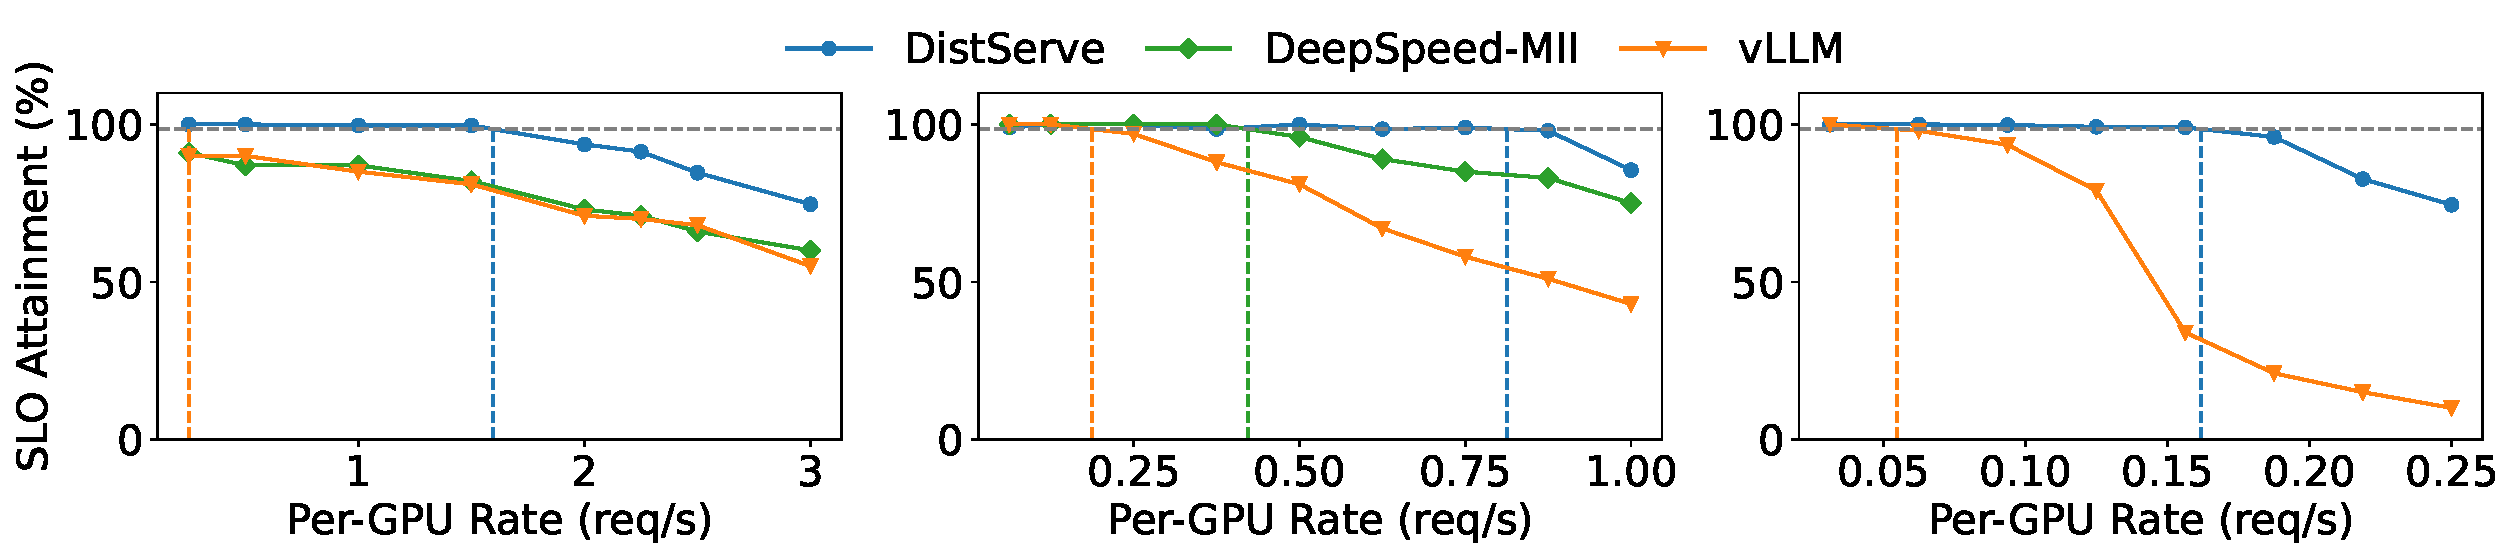
\includegraphics[width=0.95\linewidth]{figures/evaluation/chatbot-rate-p99.pdf}
    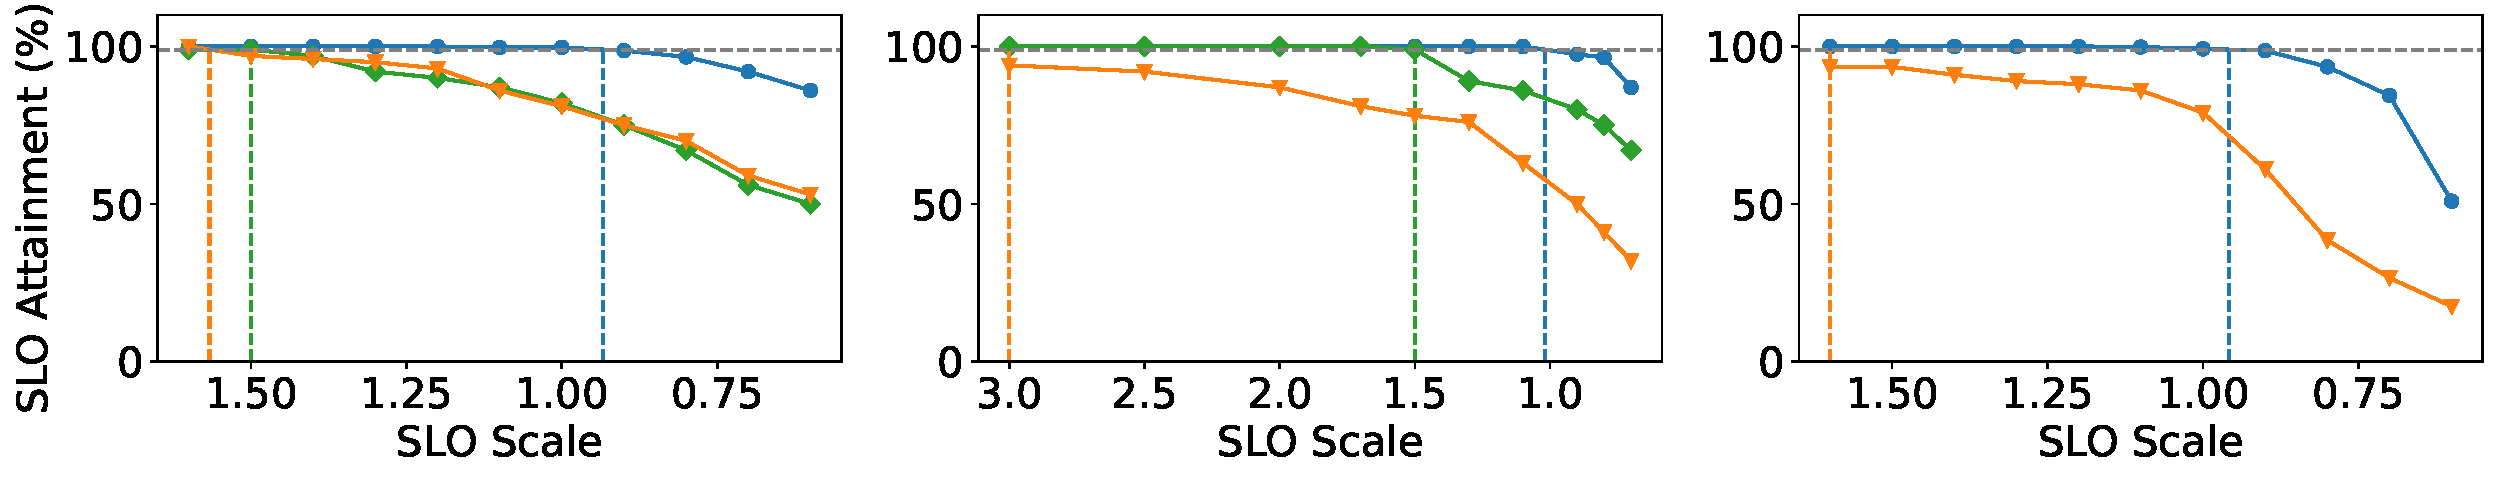
\includegraphics[width=0.95\linewidth]{figures/evaluation/chatbot-SLO-p99.pdf}
    \hspace{10mm} (a) OPT-13B \hspace{40mm} (b) OPT-66B \hspace{40mm} (C) OPT-175B
    \caption{Chatbot application with OPT models on the ShareGPT dataset.}
    \label{fig:chatbot_p99}
\end{figure*}

\begin{figure*}[!t]
    \centering
    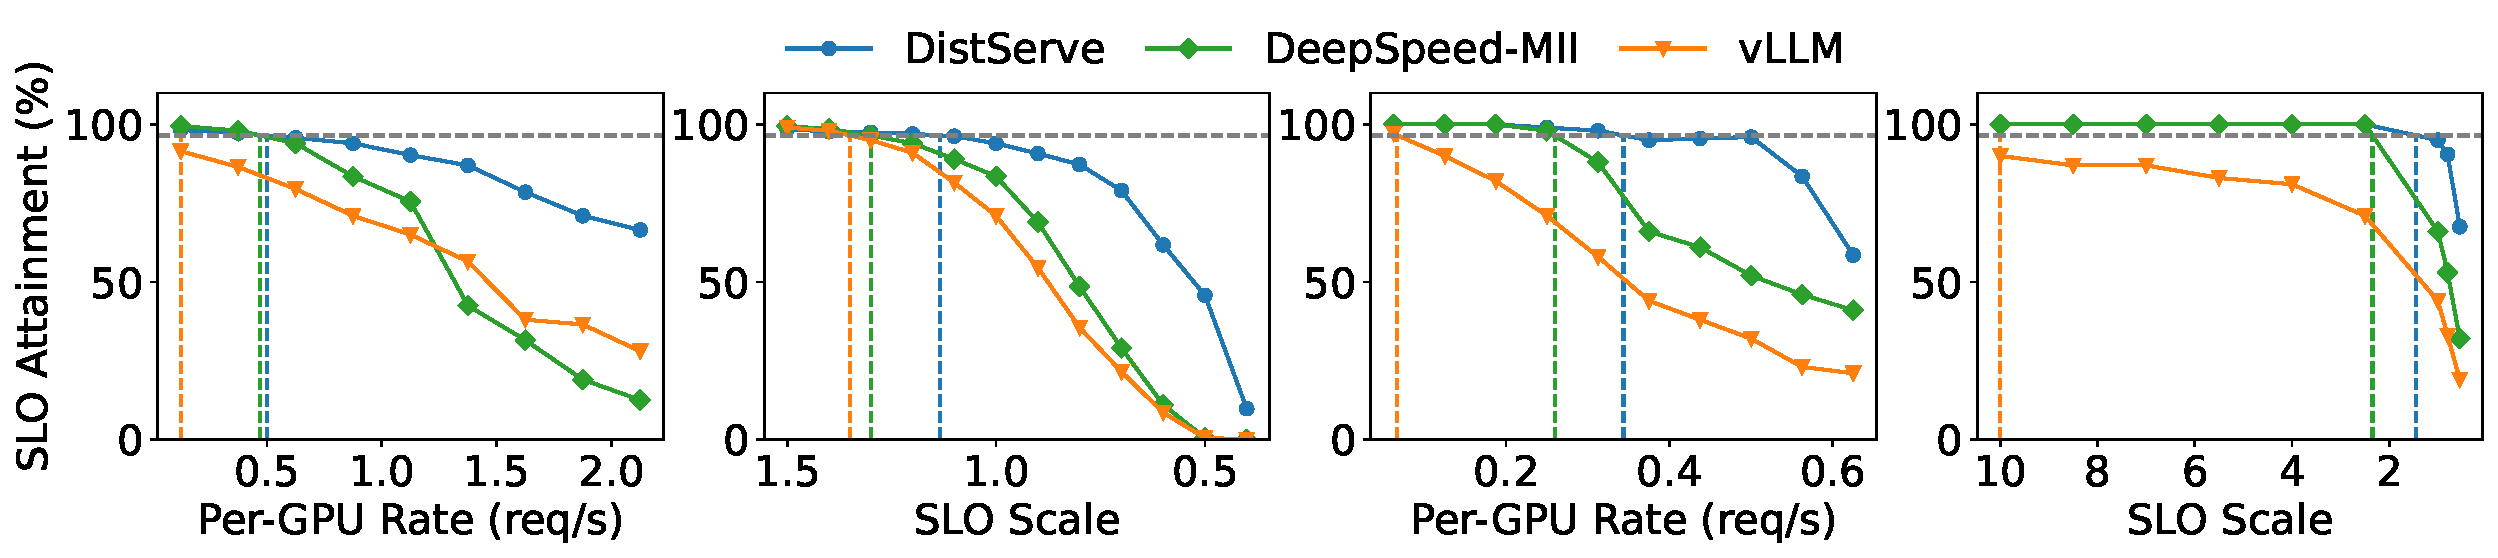
\includegraphics[width=0.95\linewidth]{figures/evaluation/other-apps-p99.pdf}
    \hspace{10mm} (a) Code Completion \hspace{50mm} (b) Summarization
    \caption{Code completion and summarization tasks with OPT-66B on HumanEval and LongBench datasets, respectively.}
    \label{fig:other_apps_p99}
\end{figure*}


\section{\sys Placements in End-to-end Experiments}
\label{appendix:placement_strategies}

Table~\ref{tab:parallel_config} shows the tensor parallelism (TP) and pipeline parallelism (PP) configurations for prefill and decoding instances chosen by \sys in the end-to-end experiments \S\ref{exp:end_to_end}.


\begin{table}[h]
\begin{tabular}{|c|c|c|c|c|c|}
    \hline
    \multirow{2}{*}{Model} & \multirow{2}{*}{Dataset} & \multicolumn{2}{c|}{Prefill} & \multicolumn{2}{c|}{Decoding} \\ \cline{3-6}
    & & TP & PP & TP & PP \\ \hline
    OPT-13B & ShareGPT & 2 & 1 & 1 & 1 \\ \hline
    OPT-66B & ShareGPT & 4 & 1 & 2 & 2 \\ \hline
    OPT-66B & LongBench & 4 & 1 & 2 & 2 \\ \hline
    OPT-66B & HumanEval & 4 & 1 & 2 & 2 \\ \hline
    OPT-175B & ShareGPT & 3 & 3 & 4 & 3 \\ \hline
\end{tabular}
\caption{The parallelism strategies chosen by \sys in the end-to-end experiments.}
\label{tab:parallel_config}
\end{table}



\section{End-to-end Results under 99\% SLO attainment}
\label{appendix:end_to_end_p99}
Figure~\ref{fig:chatbot_p99} and Figure~\ref{fig:other_apps_p99} show the end-to-end performance between \sys and baselines with the same setup in \S\ref{exp:end_to_end} except that the SLO attainment goal is changed to 99\%. We can see that under a more stringent SLO attainment goal, compared to vLLM, \sys can still sustain $3\times$--$8\times$ higher rate and $1.24\times$--$6.67\times$ more stringent SLO. When compared to DeepSpeed-MII, \sys can achieve $1.32\times$--$8\times$ higher rate and $1.20\times$--$1.58\times$ more stringent SLO.


